% =====================================================================
% CHAPTER 2 — METHODOLOGY
% =====================================================================
\chapter{Methodology}
\label{ch:method}

\section{Datasets}
\label{sec:data}

\subsection{PRISM: the primary Hinglish corpus}
The experiments use the PRISM Hinglish hate-speech dataset \cite{prism}, a
publicly available corpus of social-media posts labelled for hate speech, with
posts in English, Hindi (Devanagari) and Hinglish (Roman script). The upstream
repository revision is pinned by SHA (\texttt{b27f83eb\ldots}), the row counts are
asserted against the dataset card at load time, and each processed split is
written to disk with a SHA-256 checksum so that the exact data behind every
number cannot drift silently.

Table~\ref{tab:prism} reports the three official splits. The corpus is close to
balanced---about 53.5\% non-hate and 46.5\% hate in every split---so accuracy
alone is not misleading here, but macro-averaged metrics are still the safer
primary choice, and they are used throughout. The language distribution is the
more consequential property: by design, a substantial fraction of the corpus is
Roman-script Hinglish, which is the segment that standard tooling handles worst.

\begin{table}[htbp]
\centering
\caption[PRISM splits and label balance]{PRISM splits and label balance (verified against the pinned revision).}
\label{tab:prism}
\small
\begin{tabular}{lrrrr}
\toprule
Split & Posts & Non-hate (\%) & Hate (\%) & Purpose \\
\midrule
Train & 17{,}704 & 53.5 & 46.5 & Model fitting \\
Validation & 2{,}950 & 53.6 & 46.4 & All decisions \\
Test & 8{,}852 & 53.5 & 46.5 & Reporting only \\
\midrule
Total & 29{,}506 & 53.5 & 46.5 & \\
\bottomrule
\end{tabular}
\end{table}

Class share also varies by language. In the training split, English posts are
exactly balanced (50.0\% / 50.0\%), Hindi posts lean non-hate (55.2\% / 44.8\%),
and Hinglish posts lean non-hate most strongly (61.2\% / 38.8\%). Any
per-language comparison in Chapter~\ref{ch:results} must be read against these
different base rates.

\subsection{L3Cube-MeHate: the transfer set}
For the cross-lingual probe we use L3Cube-MeHate \cite{mehate}, a Marathi and
Marathi--English code-mixed hate-speech corpus. Only its small code-mixed
\emph{test} split is used---416 posts, 50\% / 50\% balanced---and only in zero-shot
mode: no training, no validation, no threshold re-tuning. The GitHub commit is
pinned (\texttt{8ee29fa\ldots}) and the sentiment and profanity columns shipped
with the file are deliberately ignored, keeping the label space identical to
PRISM's. Both the small split size and the single-test-split usage are stated
here as disclosed limitations rather than hidden choices.

\section{De-identification}
\label{sec:deid}

Social-media text carries personally identifiable information, and a hate-speech
corpus is exactly where it concentrates. Before any analysis, five
regular-expression rules are applied to every post of every split
(Table~\ref{tab:deid}). The rules are deliberately conservative: emojis are kept
(they are signal in this task), digit runs survive unless they look like phone
numbers, and letter elongation is collapsed for alphabetic characters only
(\emph{sooooo} $\rightarrow$ \emph{soo}).

\begin{table}[htbp]
\centering
\caption{De-identification rules applied to all splits.}
\label{tab:deid}
\small
\begin{tabular}{llp{6.2cm}}
\toprule
Pattern & Replacement & Notes \\
\midrule
URL / \texttt{www.} & \texttt{<URL>} & http(s) and bare domains \\
Email address & \texttt{<EMAIL>} & standard address pattern \\
Phone number & \texttt{<PHONE>} & $\geq$8 digits incl.\ separators \\
\texttt{@handle} & \texttt{<USER>} & mentions removed \\
Letter elongation & doubled letter & alphabetic runs only \\
\bottomrule
\end{tabular}
\end{table}

One caveat must be stated: the de-identification is regex-based, so full names
written in plain text are \emph{not} removed. This is recorded in the data card
written next to the processed splits, and it is why the processed CSVs are treated
as sensitive artifacts rather than publishable data.

\section{Exploratory Analysis and the Code-Mixing Metric}
\label{sec:eda}

\subsection{Class balance and text length}
Class share varies by language (Figure~\ref{fig:classbalance}): in the training
split, English posts are exactly balanced (50.0\% / 50.0\%), Hindi posts lean
non-hate (55.2\% / 44.8\%), and Hinglish posts lean non-hate most strongly
(61.2\% / 38.8\%). Length adds a second asymmetry: non-hate posts are longer on
average (mean 32.4 words, median 19, maximum 300) than hate posts (mean 23.7,
median 16, maximum 295), consistent with the short, direct register of abusive
attacks. Both properties matter later: any per-language comparison in
Chapter~\ref{ch:results} must be read against these different base rates, and
length is a weak but real cue that must not be confused with language effects.

\begin{figure}[htbp]
\centering
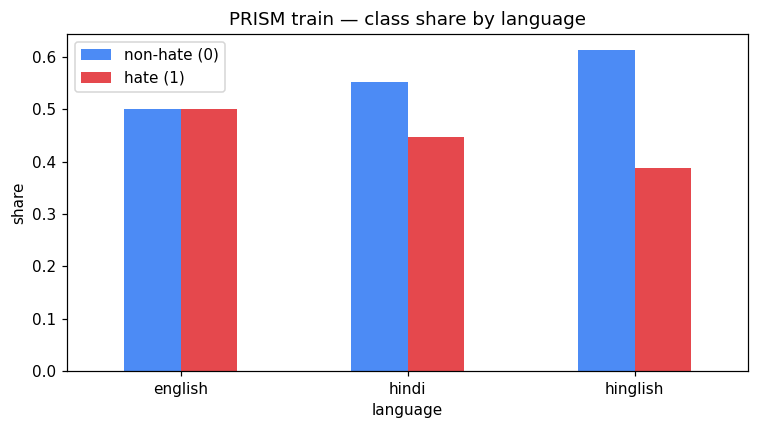
\includegraphics[width=0.62\textwidth]{figures/fig_class_balance.png}
\caption{PRISM training split---class share by language. Hinglish posts lean
non-hate (61.2\% / 38.8\%) while English posts are exactly balanced.}
\label{fig:classbalance}
\end{figure}

\subsection{Measuring code-mixing at the word level}
\label{sec:mixing}
Quantifying ``how mixed is this post'' is a prerequisite for the error analysis in
Chapter~\ref{ch:results}, and the obvious script-based measure is blind here: v1
of the pipeline measured the Devanagari character ratio, which by definition
assigns Romanised Hinglish a mixing score of exactly zero. Version 2 therefore
classifies each word token as Hindi or English: Devanagari tokens count as Hindi,
tokens in a compact romanised-Hindi lexicon (function words, common adverbs, and
frequent content terms including profanity, with common transliteration variants)
count as Hindi, and the remaining Latin tokens count as English. Placeholder
tokens and punctuation are excluded so that they cannot create phantom switches.

From these token labels the pipeline computes four statistics per post:
the Hindi token ratio; the \emph{mixing index}, defined as the minority-language
token share $\mathrm{MI} = \min(n_{\mathrm{hi}}, n_{\mathrm{en}})/n$ (0 for
monolingual text, 0.5 for a balanced mix); the number of adjacent word-level
code-switch points; and the Devanagari character ratio, kept as a script
covariate. The lexicon approach has a stated bias: content words absent from the
lexicon are counted as English, so the mixing index is a \emph{lower bound} on
true mixing.

The measurements confirm the metric can see the phenomenon
(Table~\ref{tab:mixing}). Romanised Hinglish posts average a mixing index of 0.307
with 8.5 word-level switch points per post, while pure-English posts average 0.062
(their Hindi share comes from unambiguous romanised tokens such as \emph{yaar}) and
pure-Hindi posts are exactly monolingual. Mixing is also mildly class-linked:
within Hinglish, non-hate posts mix slightly more (0.325) than hate posts (0.279),
and Figure~\ref{fig:codemixing} shows the full distributions.

\begin{table}[htbp]
\centering
\caption[Code-mixing statistics by language]{Code-mixing statistics by language (training split, means per post).}
\label{tab:mixing}
\small
\begin{tabular}{lrrr}
\toprule
Language & Hindi token ratio & Mixing index & Switch points \\
\midrule
English & 0.062 & 0.062 & 5.07 \\
Hindi & 1.000 & 0.000 & 0.00 \\
Hinglish & 0.323 & 0.307 & 8.47 \\
\bottomrule
\end{tabular}
\end{table}

\begin{figure}[htbp]
\centering
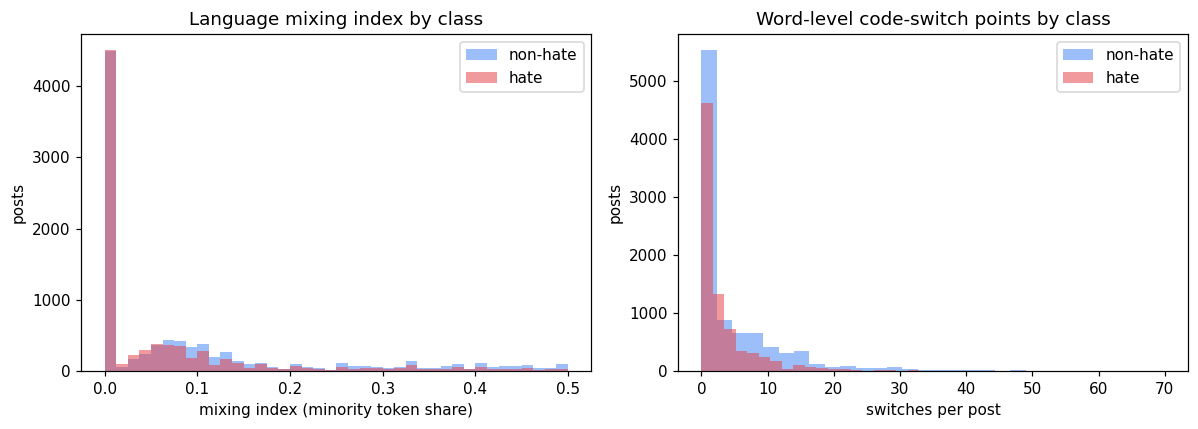
\includegraphics[width=0.8\textwidth]{figures/fig_code_mixing.png}
\caption{Language-mixing index (left) and word-level code-switch points (right)
by class. Romanised Hinglish is now visible to the metric; in v1 it scored zero.}
\label{fig:codemixing}
\end{figure}

\section{Models}
\label{sec:models}

Four classifiers are compared under one protocol. They are deliberately chosen to
span the design space from ``no learning beyond counting'' to ``pretraining on
exactly this language mixture''.

\subsection{B0 --- character $n$-gram TF-IDF + linear SVM}
The baseline vectorises each post with character $n$-grams ($n = 2$ to 5),
lowercased, minimum document frequency 2, at most 300{,}000 features with
sublinear TF weighting, and classifies with a linear support vector machine
($C = 1.0$) \cite{sklearn}. Character features are the classical answer to
romanisation noise---\emph{hain}, \emph{he} and \emph{hn} match through shared
substrings instead of exact word identity---and the model trains on CPU in
seconds. It is deterministic given the seed; its three seed runs produce
identical predictions.

\subsection{A0 --- three fine-tuned transformers}
The three transformer classifiers share the \texttt{AutoModelForSequenceClassification}
harness with a freshly initialised binary classification head, differing only in
the pretrained checkpoint that is loaded
(Table~\ref{tab:models}). The trio tests the ``does pretraining domain matter''
question: HingRoBERTa was further pretrained on $\sim$1B tokens of romanised
Hindi--English text and is the domain-matched candidate \cite{hingroberta,nayak2022};
MuRIL was pretrained on Indian-language corpora including Devanagari Hindi and is
the script-matched candidate \cite{muril}; XLM-RoBERTa is the 100-language
generalist with no special exposure to Hinglish \cite{xlmr}. All heads are trained
from scratch on PRISM; only the encoder weights come from pretraining.

\begin{table}[htbp]
\centering
\caption[The four models and their parameter counts]{The four models. ``Params'' is the fine-tuned parameter count.}
\label{tab:models}
\small
\begin{tabular}{p{2.6cm}p{4.6cm}rp{3.4cm}}
\toprule
Model & Checkpoint & Params & Rationale \\
\midrule
B0 & TF-IDF char 2--5 grams + LinearSVC & --- & Lexical control; CPU; noise-robust \\
HingRoBERTa & \texttt{l3cube-pune/hing-roberta} & 278.0\,M & Pretrained on romanised Hinglish \\
MuRIL & \texttt{google/muril-base-cased} & 237.6\,M & Indian languages, Devanagari-strong \\
XLM-RoBERTa & \texttt{xlm-roberta-base} & 278.0\,M & 100-language generalist \\
\bottomrule
\end{tabular}
\end{table}

\section{Training Protocol}
\label{sec:training}

All transformer runs use one training loop and one hyperparameter set
(Table~\ref{tab:hyperparams}), so no model can win by configuration shopping. The
checkpoint restored at the end of training is the one with the best
\emph{validation} macro-F1, not the last epoch, and fp16 mixed precision is
enabled on GPU.

\begin{table}[htbp]
\centering
\caption[Training configuration shared by all transformer runs]{Training configuration shared by all transformer runs (full-run mode).}
\label{tab:hyperparams}
\small
\begin{tabular}{ll}
\toprule
Setting & Value \\
\midrule
Maximum sequence length & 128 subword tokens \\
Epochs & 3 \\
Batch size (train / eval) & 32 / 64 \\
Learning rate & $2\times10^{-5}$ (AdamW) \\
Weight decay / warmup ratio & 0.01 / 0.1 \\
Precision & fp16 on GPU \\
Seeds & 42, 43, 44 (seeded in torch and HF) \\
Checkpoint selection & Best validation macro-F1 \\
Logging / reporting & every 50 steps / none (files only) \\
\bottomrule
\end{tabular}
\end{table}

Three implementation choices deserve note because they protect the results rather
than decorate them. First, the three seeds are genuine repetitions: seed 42's
artifacts are kept resident for the error analysis, while seeds 43 and 44 are
trained, scored, and explicitly deleted from GPU memory before the next run.
Second, predictions of every run are saved as arrays before any metric is
computed, so the significance tests later reuse exactly the training-time outputs.
Third, a smoke-test mode (tiny model, four optimiser steps, CPU-allowed) lets the
full pipeline be exercised end-to-end in about two minutes before spending GPU
hours; a fail-fast assertion refuses the full run when no GPU is present, because
a CPU run would silently drop fp16 and change the experiment.

\section{Evaluation Protocol and Metrics}
\label{sec:protocol}

\subsection{Metrics}
Five dataset-level metrics are computed for every run: macro precision, macro
recall, macro-F1, the Matthews correlation coefficient (MCC) and balanced
accuracy. \emph{Macro-F1} is the single primary metric: it averages the F-scores
of the two classes equally, so a model cannot hide a collapsing minority class
behind the majority one. MCC and balanced accuracy are robustness checks---MCC
summarises the whole confusion matrix, balanced accuracy exposes recall imbalance.
Per-class scores are analysed in \S\ref{sec:perclass}; formal definitions of
every metric are collected in Appendix~A.

\subsection{The decision threshold is a tuned parameter}
The transformers output class probabilities, and the default rule ``predict hate
if $p \geq 0.5$'' is itself a modelling choice. The pipeline therefore sweeps the
threshold from 0.05 to 0.95 in steps of 0.01, evaluates macro-F1 at each value
\emph{on the validation set only}, and carries the argmax threshold to the test
set. Chosen thresholds ranged from 0.46 to 0.53 across the nine runs---a range
that brackets 0.5 without being centred on it; Section~\ref{sec:threshold}
quantifies how much the tuning matters. The baseline is unaffected: a linear SVM
has no probability output, so its boundary is fixed.

\subsection{Which numbers may be used for which decision}
The protocol distinguishes three information channels, and the distinction is the
central methodological fix of v2:
\begin{itemize}
\item \textbf{Validation macro-F1} drives every decision: per-epoch checkpoint
selection, threshold tuning, and the choice of the best A0 backbone for the
error analysis and the transfer test.
\item \textbf{Test macro-F1} (3-seed mean $\pm$ standard deviation, plus a
bootstrap 95\% CI around the mean, 1{,}000 resamples \cite{bootstrap}) is for
reporting only.
\item \textbf{Significance testing} (exact McNemar \cite{mcnemar} on the seed-42
test predictions, Holm-corrected across the three comparisons \cite{holm})
answers whether each transformer beats B0, not which transformer is best.
\end{itemize}
In v1, the backbone for the error analysis was chosen on \emph{test} macro-F1; the
v1-vs-v2 ranking of the backbones differs, which is exactly the bias this fix
removes. All reported v2 numbers use the validation-selected backbone
(XLM-R, mean validation macro-F1 0.7488 vs.\ 0.7423 and 0.7363).

\section{Statistical Testing}
\label{sec:stats}

Two complementary procedures quantify uncertainty. \emph{Bootstrap confidence
intervals}: the test set is resampled with replacement 1{,}000 times; within each
resample, macro-F1 is computed for each of the three seeds and averaged, so the
interval is centred on the plotted 3-seed mean rather than on one lucky seed.
\emph{McNemar's test}: for each transformer vs.\ the baseline, the exact binomial
test is applied to the discordant pairs---the test items where exactly one of the
two models is correct---which is the appropriate test for paired predictions on a
fixed test set. Because three transformers are compared against the same baseline,
the three $p$-values are Holm-corrected; the correction is performed and reported
explicitly rather than left to the reader.

\section{Implementation Environment}
\label{sec:environment}

The full run executes in a single Kaggle notebook on an NVIDIA T4 GPU (fp16
enabled), using \texttt{transformers} $\geq$ 4.46 (for \texttt{eval\_strategy}
and \texttt{processing\_class} semantics), \texttt{datasets} $\geq$ 3.0,
\texttt{accelerate}, scikit-learn and SciPy \cite{transformers,sklearn}. Every
stage writes to one results tree (\texttt{results/}, \texttt{figures/},
\texttt{preds/}) with a \texttt{run\_manifest.json} and a
\texttt{requirements-freeze.txt} snapshot, so each number in
Chapter~\ref{ch:results} traces to a file.
